\begin{enumerate}
	\item Exercício
	
	\begin{equation*}
		x^2 + y^2 + z^2 = 16
	\end{equation*}
	\begin{equation*}
		z = \sqrt{x^2 + y^2}
	\end{equation*}
	
	\begin{figure}[htb]
		\caption{Coordenadas esféricas - Aula 02 - Exercício I}
		\label{v19_a02_e01}
		\centering
		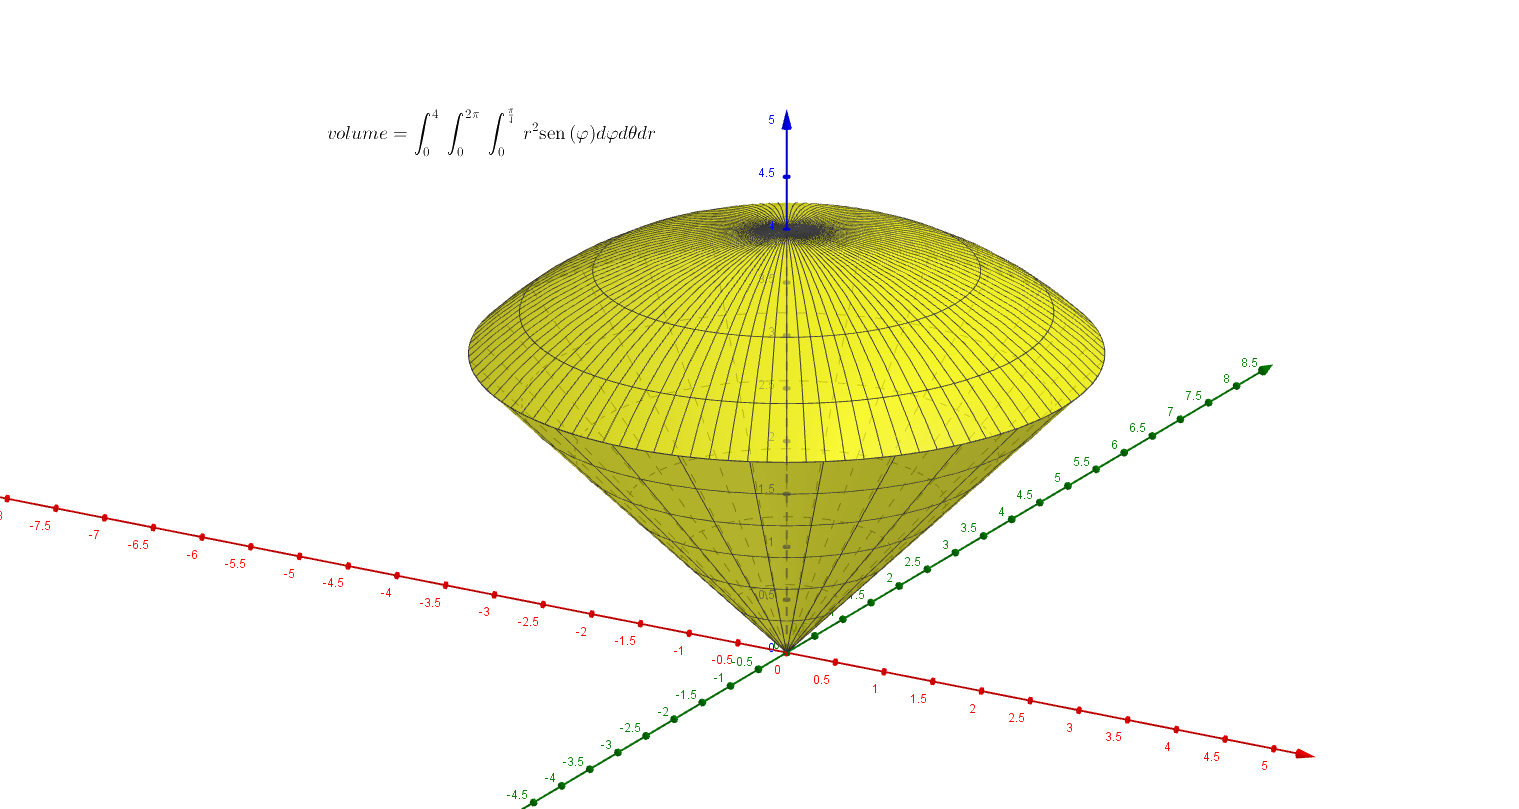
\includegraphics[width=0.5\textwidth]{v19_a02_e01.png}		
	\end{figure}
	
	\begin{gather*}
		z = \sqrt{x^2 + y^2} \Rightarrow r\cos(\varphi) = \sqrt{\left(r\sen(\varphi)\cos(\theta)\right)^2 + \left(r\sen(\varphi)\sen(\theta)\right)^2} =\\ \sqrt{r^2\sen^2(\varphi)\cos^2(\theta) + r^2\sen^2(\varphi)\sen^2(\theta)} = \sqrt{r^2\sen^2(\varphi)\left(\cos^2(\theta) + \sen^2(\theta)\right)} =\\ r\sen(\varphi) \Rightarrow \dfrac{r\cos(\varphi)}{r\cos(\varphi)} = \dfrac{r\sen(\varphi)}{r\cos(\varphi)} \Rightarrow 1 = \tg(\varphi) \Rightarrow \varphi = \arctg(1) = \dfrac{\pi}{4}
	\end{gather*}
	\begin{equation*}
		0 \leq r \leq 4,\, 0 \leq \theta \leq 2\pi,\, 0 \leq \varphi \leq \dfrac{\pi}{4}
	\end{equation*}
	\begin{gather*}
		v = \int_0^4 \int_0^{2\pi} \int_0^{\frac{\pi}{4}} r^2\sen(\varphi) d\varphi d\theta dr = \int_0^4 \int_0^{2\pi}\left(r^2\int_0^{\frac{\pi}{4}} \sen(\varphi) d\varphi\right)d\theta dr =\\ \int_0^4 \int_0^{2\pi}\left(r^2\left[-\cos(\varphi)\right]_0^{\frac{\pi}{4}}\right)d\theta dr = \int_0^4 \int_0^{2\pi}\left(r^2\left[-\cos\left(\dfrac{\pi}{4}\right) + \cos(0)\right]\right)d\theta dr =\\ \int_0^4 \int_0^{2\pi}\left(r^2\left[-\dfrac{\sqrt{2}}{2} + 1\right]\right)d\theta dr = \int_0^4 \int_0^{2\pi} \dfrac{r^2\left(2 - \sqrt{2}\right)}{2}\, d\theta dr =\\ \int_0^4 \left(\dfrac{r^2\left(2 - \sqrt{2}\right)}{2}\left[\theta\right]_0^{2\pi}\right) dr = \int_0^4 \dfrac{r^2\left(2 - \sqrt{2}\right)}{\overstrike{2}}\overstrike{2}\pi\, dr = \int_0^4 \pi\left(2 - \sqrt{2}\right)r^2\, dr =\\ \pi\left(2 - \sqrt{2}\right) \left[\dfrac{r^3}{3}\right]_0^4 = \dfrac{64\pi\left(2 - \sqrt{2}\right)}{3}
	\end{gather*}
\end{enumerate}